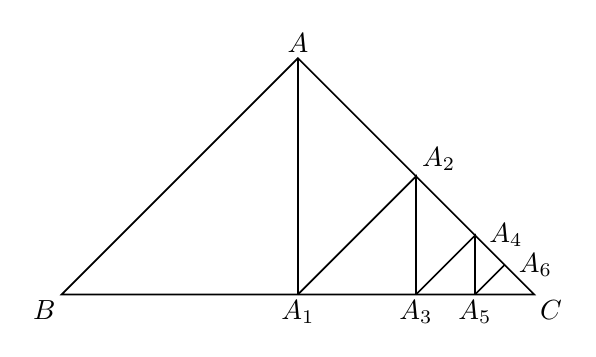
\begin{tikzpicture}[x=1cm,y=1cm,font=\normalsize,
 geometry edge/.style={solid,line width=.6pt},
 geometry mark/.style={solid,line width=.6pt},
 geometry label/.style={font=\normalsize,inner sep=2pt}]
\coordinate (A) at (3,3);
\coordinate (B) at (0,0);
\coordinate (C) at (6,0);
\coordinate (A1) at (3,0);
\coordinate (A2) at (4.5,1.5);
\coordinate (A3) at (4.5,0);
\coordinate (A4) at (5.25,0.75);
\coordinate (A5) at (5.25,0);
\coordinate (A6) at (5.625,0.375);
\draw[geometry edge] (A)--(B)--(C)--cycle;
\draw[geometry edge] (A)--(A1);
\draw[geometry edge] (A1)--(A2)--(A3);
\draw[geometry edge] (A3)--(A4)--(A5);
\draw[geometry edge] (A5)--(A6);
\node[geometry label,above] at (A) {$A$};
\node[geometry label,below left] at (B) {$B$};
\node[geometry label,below right] at (C) {$C$};
\node[geometry label,below] at (A1) {$A_{1}$};
\node[geometry label,above right] at (A2) {$A_{2}$};
\node[geometry label,below] at (A3) {$A_{3}$};
\node[geometry label,right,xshift=3pt] at (A4) {$A_{4}$};
\node[geometry label,below] at (A5) {$A_{5}$};
\node[geometry label,right,xshift=3pt] at (A6) {$A_{6}$};
\end{tikzpicture}